\documentclass[a4paper, 11pt]{article}
\usepackage[top=3cm, bottom=3cm, left = 2cm, right = 2cm]{geometry} 
\geometry{a4paper} 
\usepackage[utf8]{inputenc}
\usepackage{textcomp}
\usepackage{graphicx} 
\usepackage{amsmath,amssymb}  
\usepackage{bm}  
\usepackage{lipsum}
\usepackage[pdftex,bookmarks,colorlinks,breaklinks]{hyperref}  
%\hypersetup{linkcolor=black,citecolor=black,filecolor=black,urlcolor=black} % black links, for printed output
\usepackage{memhfixc} 
\usepackage{pdfsync}   
\usepackage{fancyhdr}
\usepackage{hyperref}
\usepackage{tikz} 
\usepackage{seqsplit}
\usepackage{listings,xcolor}
\usetikzlibrary{positioning}

\pagestyle{fancy}

\title{Native Smart Contract}
\author{Phan Dinh Minh Hieu}
%\date{}

\begin{document}
\maketitle
\tableofcontents
\pagebreak

\section{Introduction}

Native Smart Contracts are smart-contract belong to the core blockchain. 
These smart contracts will be executed by the root node and its storage will be saved in the validators and nodes
instead of the storage node.
\section{Flow}
\subsection{Execute}
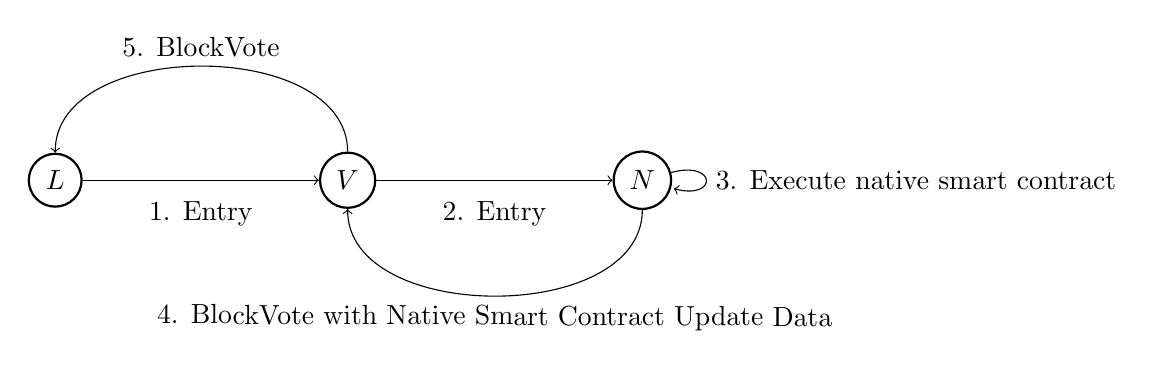
\begin{tikzpicture}[node distance={30mm}, main/.style = {circle, thick, draw}]
    \node[main] (1) {$V$}; 
    \node[main] (2) [right=30mm of 1] {$N$}; 
    \node[main] (3) [left=30mm of 1]{$L$}; 
    \path[->] (3) edge node[below =0.15 cm] {1. Entry} (1);
    \path[->] (1) edge node[below =0.15 cm] {2. Entry} (2);
    \path (2) edge [loop right] node[right] {3. Execute native smart contract} (2);
    \path[->] (2) edge[bend left = 90] node[midway, below, sloped] {4. BlockVote with Native Smart Contract Update Data} (1);
    \path[->] (1) edge[bend right = 90] node[midway, above, sloped] {5. BlockVote} (3);
\end{tikzpicture} 

\subsection{Confirm}
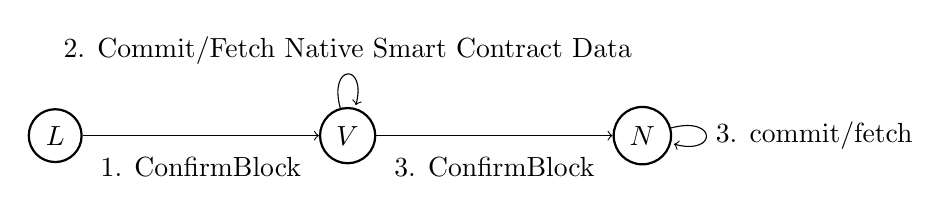
\begin{tikzpicture}[node distance={30mm}, main/.style = {circle, thick, draw}]
    \node[main] (1) {$V$}; 
    \node[main] (2) [right=30mm of 1] {$N$}; 
    \node[main] (3) [left=30mm of 1]{$L$}; 
    \path[->] (3) edge node[below =0.15 cm] {1. ConfirmBlock} (1);
    \path[->] (1) edge node[below =0.15 cm] {3. ConfirmBlock} (2);
    \path (1) edge [loop above] node[above] {2. Commit/Fetch Native Smart Contract Data} (1);
    \path (2) edge [loop right] node[right] {3. commit/fetch} (2);
\end{tikzpicture} 

\subsection{Sync}
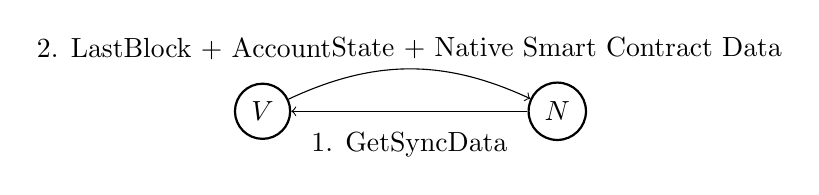
\begin{tikzpicture}[node distance={30mm}, main/.style = {circle, thick, draw}]
    \node[main] (1) {$V$}; 
    \node[main] (2) [right=30mm of 1] {$N$}; 
    \path[->] (2) edge node[below =0.15 cm] {1. GetSyncData} (1);
    \path[->] (1) edge[bend left = 25] node[midway, above, sloped] {2. LastBlock + AccountState + Native Smart Contract Data} (2);
\end{tikzpicture} 


% \begin{tikzpicture}[node distance={30mm}, main/.style = {circle, thick, draw}]
%     \node[main] (1) {$L$}; 
%     \node[main] (2) [left=30mm of 1] {$V$}; 
%     \node[main] (3) [right=30mm of 1] {$V$}; 

%     \path[->] (1) edge node[below =0.15 cm] {1. Entry} (2);
%     \path[->] (1) edge node[below =0.15 cm] {1. Entry} (3);

%     \node[main] (4) [below=45mm of 3] {$pN$}; 
%     \path[->] (3) edge[bend right = 25] node[midway, above, sloped] {2. Entry} (4);
%     \path (4) edge [loop left] node[left] {3. VerifyPacksSignAndData} (4);

%     \node[main] (5) [ above right=30mm and 45mm of 4] {$vM$}; 
%     \path[->] (4) edge[bend left = 25] node[midway, below, sloped] {4. VerifyPacksSign} (5);
%     \path[->] (5) edge[bend left = 25] node[midway, below, sloped] {5. VerifyPacksSignResult} (4);


%     \node[main] (6) [below=65mm of 4] {$N$}; 
%     \path[->] (4) edge[bend right = 25] node[midway, below, sloped] {6. VerifyPacksSign} (6);

%     \node[main] (7) [below left=65mm of 6] {$vM$}; 
%     \path[->] (6) edge[bend right = 25] node[midway, above, sloped] {7. VerifyPacksSign} (7);
%     \path[->] (7) edge[bend right = 25] node[midway, below, sloped] {8. VerifyPacksSignResult} (6);


%     \path[->] (6) edge[bend left = 90] node[midway, below, sloped] {9. VerifyPacksSignResult } (4);
%     \path[->] (4) edge[bend left = 25] node[midway, below, sloped] {10. ExecuteTransactions} (6);


%     \node[main] (7) [below right=65mm of 6] {$eM$}; 

%     \path[->] (6) edge[bend right = 25] node[midway, below, sloped] {11. ExecuteTransactions} (7);
%     \path[->] (7) edge[bend right = 25] node[midway, above, sloped] {12. ExecuteTransactionsResult} (6);
%     \path[->] (6) edge[bend right = 90] node[midway, below, sloped] {13. ExecuteTransactions} (4);

%     \path (4) edge [loop above] node[left] {14. Update account state and create block vote} (4);

%     \path[->] (4) edge[bend right = 25] node[midway, below, sloped] {15. NodeBlockVote} (3);
%     \path[->] (3) edge[bend right = 25] node[midway, above, sloped] {16. ValidatorBlockVote} (1);
% \end{tikzpicture} 

\section{Reward Smart Contract}

\bibliographystyle{abbrv}
% \bibliography{references}  % need to put bibtex references in references.bib 
\end{document}